%!TEX root = ../thesis.tex
\chapter{Literature Review} % (fold)
\label{cha:literature_review}

Due to limited work and constraint of availability of relevant literature with regards to our scenario we took a 3-part approach to our literature i.e.
\begin{itemize}
    \item Literature on ASR in English Language.
    \item Literature on Languages relevant to Urdu i.e. Arabic and Hindi.
    \item Literature specific to ASR implementation in Urdu Language - A low resourced language.
\end{itemize}

\section{Literature on English Language}

There is ample amount of literature on English ASR available. In fact all state-of-the-art Training methods from Traditional ASR to Hybrid HMM-DNN to modern E2E Systems are thoroughly tested on English Language with WERs $<6\%$. 

\cite{dahl_context-dependent_2012} first introduced HMM–DNN hybrid approach in which Deep neural network model replaced GMM which increased accuracy compared to traditional HMM-GMM legacy system. They achieved 5.8\% and 9.2\% absolute sentence accuracy improvement or 16.0\% and 23.2\% relative error reduction over the CD-GMM-HMMs trained respectively using the minimum phone error rate (MPER) and maximum-likelihood (ML) criterion on Bing Voice Search Business English Dataset with 24 hours of training set (32057 utterances), 6.5 hours of Dev Set (8777 utterances) and 9.5 hours of Test Set (12758 utterances). The data-set had variations like noise, music, side-speech, accents, sloppy pronunciation, hesitation, repetition, interruption, and different audio channels. This however would require us to build our own code-switched Language model based on our own corpus.

\cite{georgescu_performance_2021} studied and compared the performance of Hybrid HMM-DNN and Deep Learning based methods trained on English LibriSpeech data-set of 1000hours, which showed that Hybrid HMM-DNN based systems, particularly TDNN and CNN-TDNN outperformed End to End Methods with WER of 3.85\% and 3.87\% respectively with least memory load of 106 MB for loading NN model and storing all the activation's of the network for processing per second of speech which supports the conclusion by \cite{christian_gaida_comparing_2014} and \cite{naeem_subspace_2020}. This model was however not trained on noisy telephonic data which is why it is not applicable for our scenario. Moreover, it was trained only on English and our language modelling would different and irrelevant for our code-switched Urdu scenario.  

\cite{smit_advances_2021} implemented sub-word units in using DNN based acoustic and RNN based language models trained on on 283 hours of English Data-set which resulted in WER of 18\% which was too high for our use. 

\section{Literature on Languages relevant to Urdu i.e. Arabic and Hindi}
For greater insights, we selected two of the languages that were closest in structure (written and spoken) to Urdu Language; Arabic and Hindi. There was ample amount of research available in these languages which helped cover up for the shortcomings in the research pertaining to Urdu ASR, particularly the code-switched version.

\subsection{Arabic Language}
Arabic is one of the most actively researched language in ASR field. \cite{khurana_qcri_2016} merged three acoustic models trained with LFMMI objective function using similar architecture as \cite{povey_purely_2016} on 1200 hours of Dialectical Arabic MGB-2 data-set. They merged TDNN, LSTM, and BLSTM using the Minimum Bayes Risk decoding criterion, achieving WER of 14.2\%. 

Ali Et al (2017) from Aalto University \cite{ali_speech_2017} merged 30-plus systems using MBR, including two acoustic models TDNN-BLSTM along with variety of language models like character-based, sub-word, and word-based \cite{smit_aalto_2017}. 13.2\% WER was achieved on MGB-2 which was a 10\% improvement compared to results of 2016, and 37.5\% average WER and 29.3\% multi-reference WER was achieved on MGB-3. These were based on Arabic language and not applicable for our uses. Moreover, Arabic is far more resourceful compared to Urdu which is why we could not use this for our Code-Switched Urdu environment. 

\cite{alsayadi_arabic_2021} conducted training of Models in Traditional ASR and E2E ASR using 1200 hours of Arabic Speech Corpus \cite{alhanai_development_2016}.
Eight models for traditional ASR have been used, four of which use GMM, two of which use SGMM, and the last two models use DNN. End-to-end methods for diacriticised Arabic ASR were used which are based on CTC-attention and CNN-LSTM. WER of 33.72\% on conventional ASR and 28.5\% on CNN-LSTM. The drawback of this for our case was that training a model like this needed 1000 of hours of labelled data for training and that volume of labelled code-switched Urdu data was not available to us.

\cite{hussein_arabic_2022} comprehensively performed  bench-marking for E2E transformer, modular HMM–DNN, and human speech recognition on the Dialectical Arabic. End-to-end ASR gave 12.5\%, 27.5\% , 33.8\% WER on MGB-2, MGB-3, and MGB-5 data-sets respectively. The drawback is that we did not have labelled data for code-switched Urdu to conduct this kind modelling. %Their results also showed that human performance in the Arabic language is still considerably better than the machine with an absolute WER gap of 3.5\% on average.

\begin{figure}[h!]
    \centering
    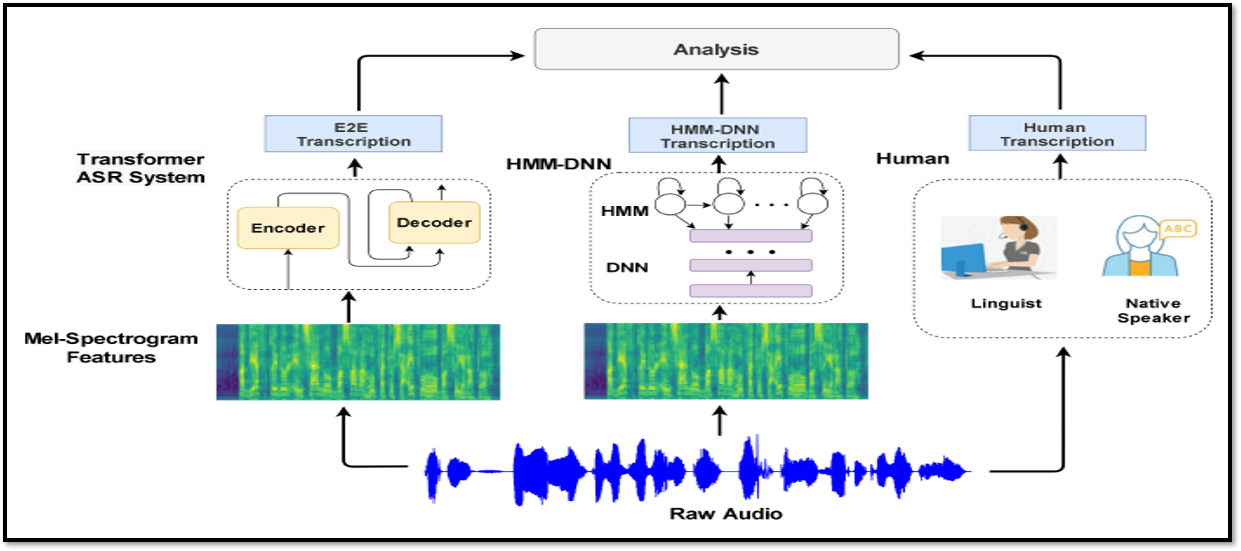
\includegraphics[scale=0.40]{img/ASR-diagram-comparison.png}
    \caption{E2E vs Hybrid DNN-HMM vs HSR \cite{hussein_arabic_2022}}
    \label{fig:hybrid-vs-e2e-HSR}
\end{figure}

\subsection{Hindi Language}
The majority of work in the field of speech recognition in South Asian Languages has been done on Hindi, which is very similar to spoken Urdu \cite{farooq_improving_2019} \cite{dash_automatic_2018}. Isolated word recognition \cite{patil_automatic_2016}, connected digit recognition \cite{a_n_mishra_robust_2011}, statistical pattern classification \cite{aggarwal_using_2011}, online speech to text engine \cite{b_venkataraman_sopc-based_2006} and large vocabulary speech recognition systems have been developed in Hindi \cite{kumar_large-vocabulary_2004}. 

On the AMUAV Hindi speech database, Upadhyaya \cite{tanveer_continuous_2019} developed a Hindi speech recognition system using deep neural networks. This database contains 1000 phonetically balanced sentences recorded by 100 different speakers and covers 54 different Hindi phones. Using DNN implementation by \cite{karel_vesel_sequence-discriminative_2013}, the minimum achieved WER was 11.63\% which is high for our use.

Lakhshmi's \cite{lakshmi_sri_kaldi_2020} work involved training a data-set of 158 Hindi medical terms from 16 female and 11 male speakers, almost 3 hours of data, audio sampled at 16KHz, single channel. Best WER of 2\% was achieved using Triphone Acoustic Modelling. Although this system has a low WER, it cannot be used as a replacement for Urdu ASRs due to significant differences in lexicon, pronunciations etc \cite{k_v_s_parsad_and_s_m_virk_computational_2012}.

In general, using Hindi Language Model is not the optimum solution to implement in Code-switched Urdu telephonic environment due to differences in the linguistic foundation, vocabulary, written scripts, etc which means that using Roman Hindi model for Speech to Text will not be optimal because of differences in writing and pronunciation of words e.g. the word \textit{"Zeera"} in Urdu is pronounced \textit{"Jeera"} in Hindi (in writing and in pronunciation both). Phones like \textit{"/Z/"} \textit{"/kh/"} \textit{"/gh/"} are pronounced differently in Hindi and in Urdu. This will result in low accuracy in our scenario.

\section{Literature on Urdu Language}

Urdu has about 170 million speakers \cite{ethnologue_urdu_nodate} and is spoken in India, Pakistan, Bangladesh, and many other parts of the world which is why it is important that the benefits of ASR are available in the Urdu domain. Urdu is low resourced due to scare publicly available text corpus, transcribed speech data and pronunciation lexicon. A robust ASR generally requires thousands of hours of transcribed speech data, as well as a massive text corpus and lexicon. As a result, Urdu speakers are excluded from the benefits of ASR. 

Over the years, very little efforts have been made to develop resources and speech-technology-related applications for Urdu compared to English and Arabic. Ashraf et al. 2010 \cite{hutchison_speaker_2010} pioneered the development of an isolated speech recognition system in the domain of Urdu speech recognition. The vocabulary comprised of 52 words spoken by 10 speakers. For unseen speakers, a minimum Word Error Rate (WER) of 10.6\% was achieved. This was done on limited vocabulary and has high error rate which is why it is not applicable for our use and was only tested on isolated words whereas we needed a LVCSR.

\cite{sarfraz_large_2010} developed a continuous speech recognition system in Urdu using spontaneous speech corpus collected from 82 speakers which had WER of 68.8\%. \cite{sarfraz_huda_speech_2016} recorded the speech corpus over telephone and microphone channels. The corpus duration was 45 hours, with vocabulary of 14000 words. A minimum WER of 68.8\% was attained which was too high for our use.

A speaker-independent Urdu speech recognition system was developed by Qasim \cite{qasim_urdu_2016} for 139 district names of Pakistan which covered various Pakistani accents, giving WER of 7.44\% by building adapted ASR on field data. This is not applicable for our use because it has a limited vocabulary and would not work in a noisy code-switched Urdu environment. 

Shaikh et al 2015 \cite{shaik_improvements_2015} developed an LVCSR on 99 hours of Urdu broadcast data with vocabulary of 79,000 words. A 5-gram Language Model was built with corpus of 266 Million words collected from various newspapers. Evaluation was done on 0.5 hours of data which gave WER of 32.6\% using GMM-HMM based speaker adapted system. The data set and model however is not openly available and the word error rate is too high for our use. Moreover, GMMs has a drawback of being inefficient for nonlinear class boundaries because they assume each frame is generated by a single component of the mixture which required them to be replaced by DNNs \cite{dahl_context-dependent_2012}.

Raza \cite{raza_rapid_2018} collected 1207 hours of speech dataset from 11017 speakers all over Pakistan with vocabulary of 5000 words from which 9.5 hours data was annotated and out of that, 8.5 hours were used as training dataset. Evaluation was done on 1 hour of test data which gave WER of 24.14\% which was too high for our use. 

\cite{farooq_improving_2019} developed an LVCSR using 300 hours of read-out speech data, in both indoor and outdoor environments, with a vocabulary size of 199,000 words from 1671 Urdu and Punjabi speakers. GMM-HMM, TDNN, LSTM, and Bidirectional  LSTM based Acoustic Modelling is done. For re-scoring, Recurrent Neural Network Language Model (RNNLM) was used. Evaluation was done on 9.5 hours of test data-set giving WER of 13.5\% which was too high for our use.

\cite{farooq_enhancing_2020} used 25 hours of their own Urdu speech corpus for enhancement of read-Urdu-speech LVCSR to recognize code-switched speech using the HMM-DNN modeling technique without any prior GMM-HMM training and alignments. Various techniques to improve language models using monolingual data were used giving overall percent Word Error Rate (WER) 26.95\%.

\cite{naeem_subspace_2020} developed SGMM based ASR model for continuous speech with the Data-set structured by RUMI, CSALT and FAST-NUCES. They developed a 50-hour Urdu speech data set, transcribed and merged with CSALT, ITU data-set to produce 100 hours of audio data-set. Audio files had sampling rate of 16000Hz and used mono-channel. They achieved a WER of 9.7\% with 100 hours of their data. The drawback is that data as well as the model is however not openly available and it is not tested in a telephonic audio data. 
 
Sehar Gul \cite{sehar_gul_detecting_2020} developed an ASR to detect malicious speech using Deep Speech \cite{mozilla_deep_nodate} (an End to-End ASR Engine) with 86 malicious sentences, 100 random Urdu sentences, and 250 sentences from Ali et. al 2015 \cite{ali_automatic_2015} spoken by 10 speakers, sampled at 8K mono channel. It achieved a Word Error Rate of 40\%. The drawbacks are that it was trained on Deep Learning platform with very less dataset. It was also not applicable on a noisy environment which required us to redesign the whole Speech To Text Pipeline.   

\cite{qureshi_urdu_2021} trained an ASR with the PRUS data-set  \cite{zia_pronouncur_2018} comprising of 708 sentences by 7 speakers with GMM based triphone acoustic models which gave overall recognition accuracy values 78.2\% for 100 words. This was a good baseline for us to work with since that data was available to us. %First five experiments were trained a GMM based tri-phone acoustic model on the first 600 sentences of the corpus. Sixth experiment was trained a GMM based tri-phone acoustic model on the first 600 sentences of each speakers’ corpus (combined first 600 sentences of each member to form one large training corpus) and tested it on the rest of the 108 sentences of each speaker’s corpus (combined 108 sentences of each member to form one testing corpus). Experiment 7-11 trained a GMM based tri-phone acoustic model on the complete corpus (708 sentences) of n-1 speakers and tested it on the complete corpus of the remaining 1 speaker, so 5 different models (leaving out SP1-SP5).

While the work mentioned in the preceding literature reports achievements on the Urdu ASR task, it lacks information on free corpus and does not point out corpus resources that others could adopt and use for a fair comparison. We used data-set from Ali et al 2015 \cite{ali_automatic_2015}, Sehar \cite{sehar_gul_detecting_2020} and PRUS \cite{zia_pronouncur_2018} \cite{qureshi_urdu_2021} results of which were compared with our model (\ref{sec:comparison_result}).

\section{Challenges} % (fold)
\label{sec:challenges}
Based on our literature review, we will need to build our own ASR from scratch because of lack of availability of good pre-trained models and data-sets in Urdu language for Noisy Telephonic Environment, with good WER and SER. In this regard we need:
\begin{itemize}
    \item ASR training model to train our data   
    \item Telephonic code-switched Urdu audio data-set (Mono 16000Hz) with Roman Urdu Transcript which would cater for:
    \begin{itemize}
        \item Isolated Digits
        \item Isolated words
        \item Read Speech (Words and Digits)
        \item Spontaneous Speech (Words and Digits)
        \item Clean Audio
        \item Noisy or Telephonic Audio
    \end{itemize}
    %\item Practical Implementation setup for testing our work. 
    \item Achievement of WER $<$ 10\% and SER $<$ 30\% in clean as well as in noisy environment (as well as in spontaneous, read-speech and isolated words)
\end{itemize}

%\begin{figure}[h!]
%    \centering
%    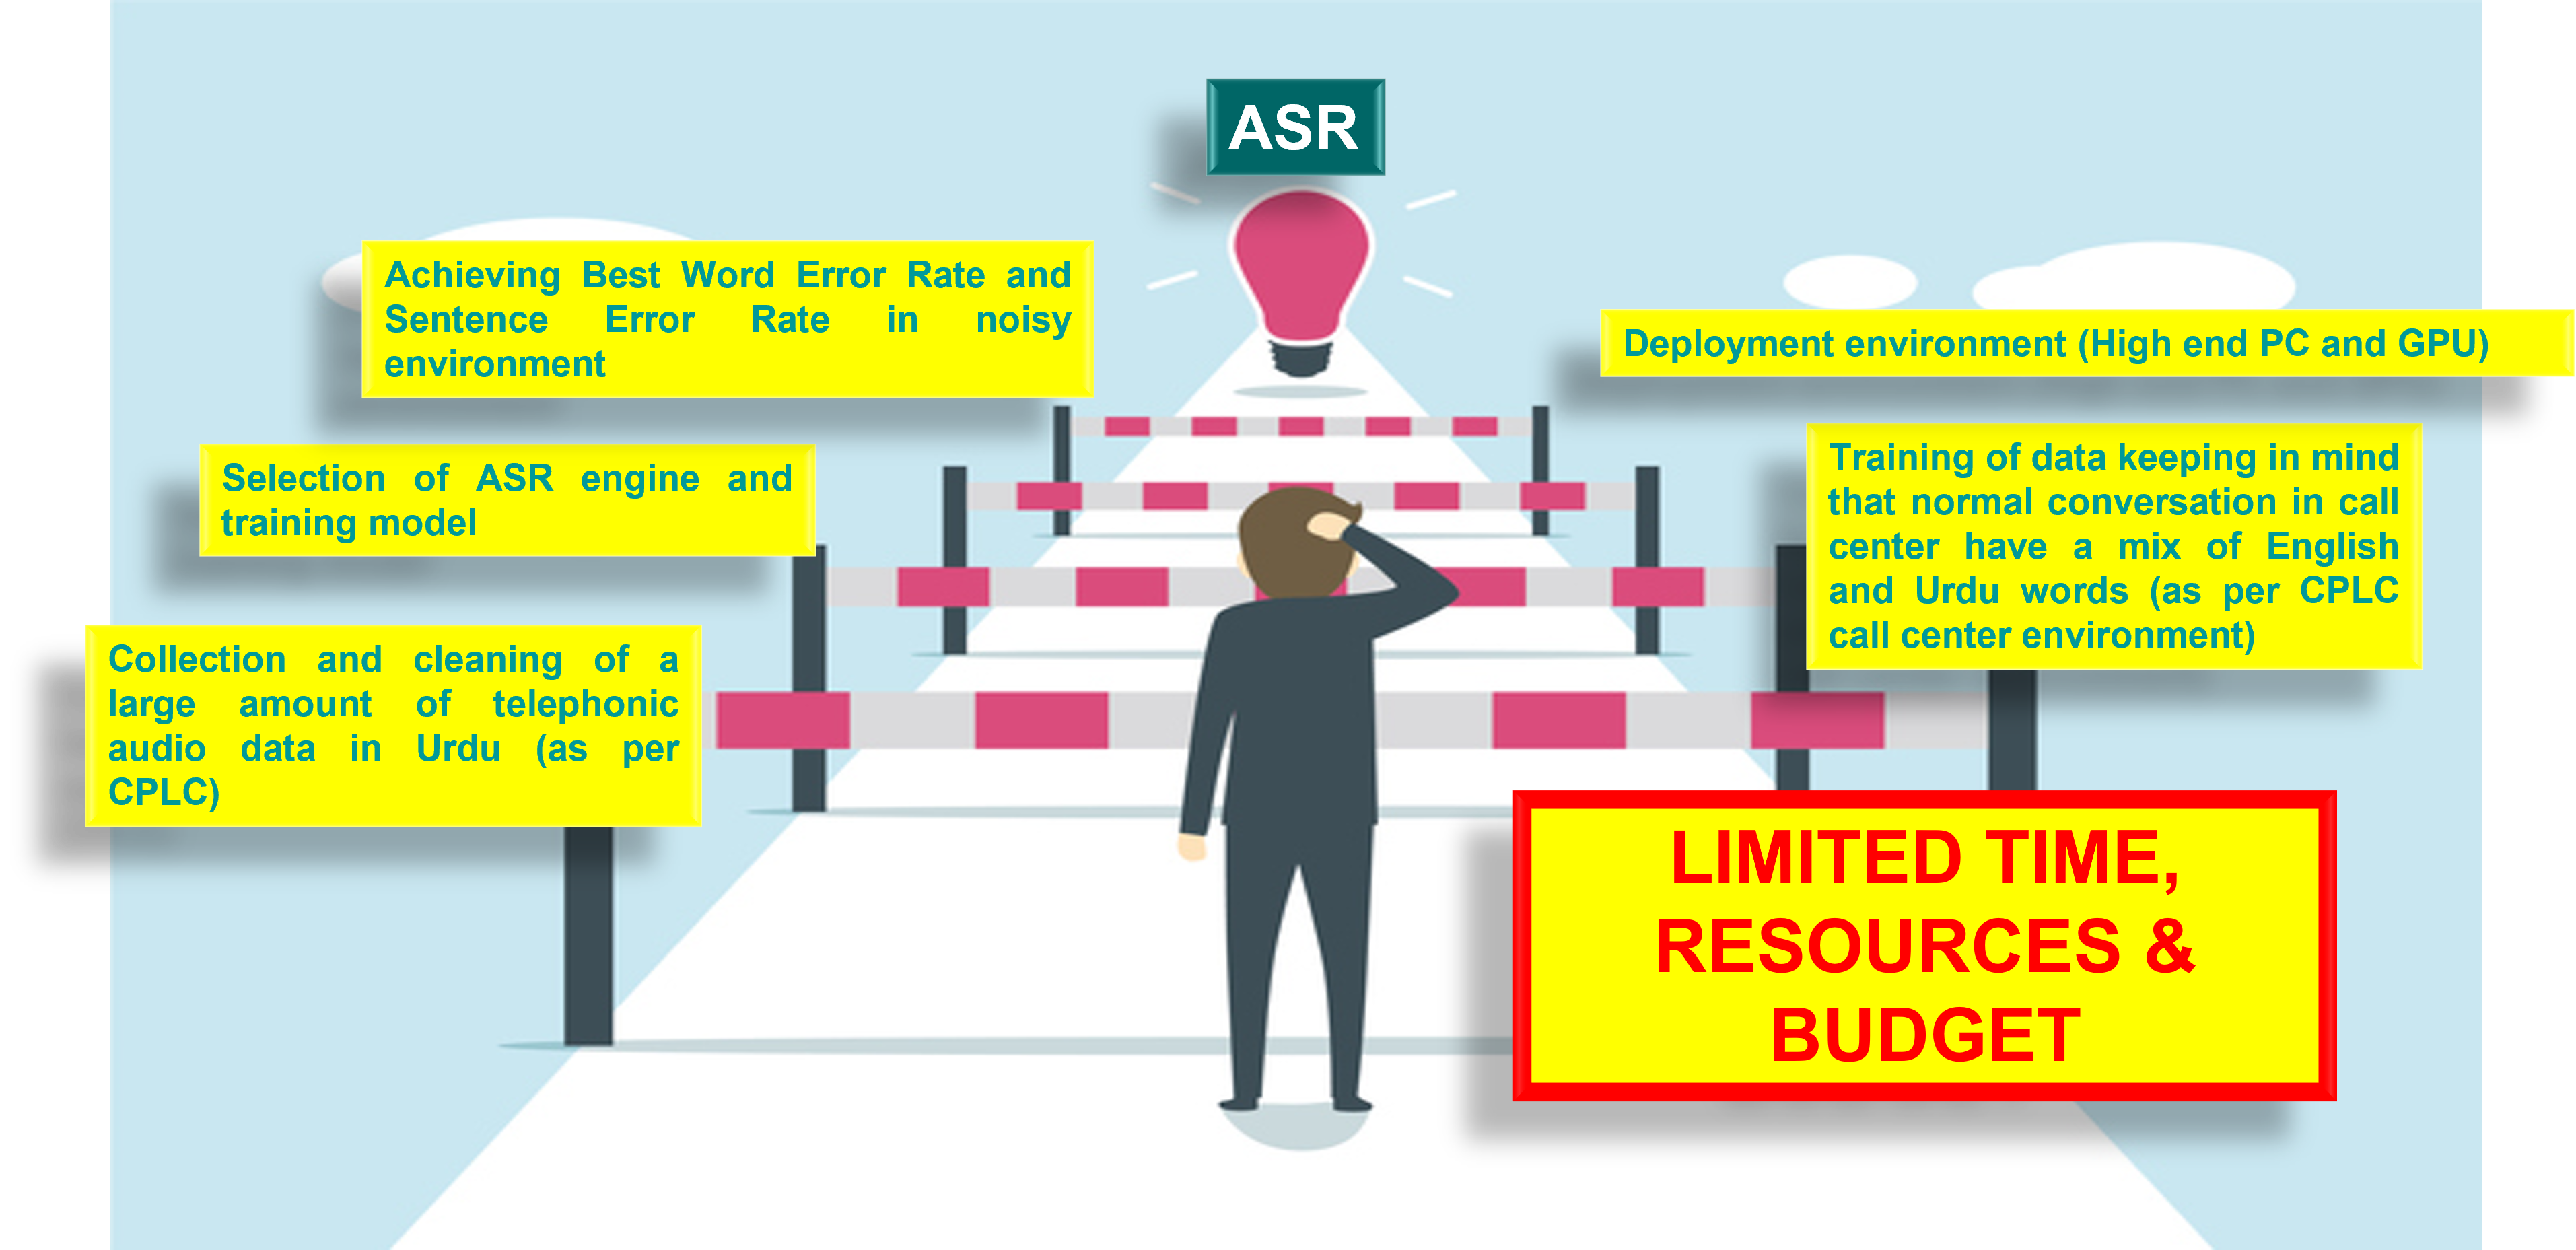
\includegraphics[scale=0.5]{img/Challenges.png}
%    \caption{Challenges to our work}
%    \label{fig:challenges}
%\end{figure}

\section{Selection of Approach for our Methodology}
The majority of AI applications are currently model-centric, a possible reason being that AI industry pays close attention to academic research on models. Since it is difficult to create large data-sets which can become widely accepted standards, more than 90\% of AI research papers are model-centric \cite{deeplearningai_data-centric_2021}. The Code becomes the major focus and data-set is frequently overlooked which is why data collection and pre-processing is considered as a one-time event.

Accenture \cite{noauthor_scaling_nodate} informs that about 85\% of projects are still proof of concept \cite{noauthor_data-centric_nodate} which are not brought into production, yet. The reason why model-centric approach of previous works have not been deployed in production environment include:

\begin{enumerate}
    \item \textbf{Requirement of highly customized solutions.} 
    \begin{itemize}
        \item Various companies e.g. manufacturing company with multiple line of products cannot apply one Model for all products to detect production errors in them, unlike advertisement companies like Google or facebook Ads.
        \item In ASR scenario, model for one language cannot work on all languages because every language needs different model. Giants like Google, Microsoft or Facebook may be able to have ML department for each product line but not every company can afford the cost of Data Scientists/ Engineers and MLOps Engineers.
    \end{itemize}
    \item \textbf{Limited points of Data Collection.} 
    \begin{itemize} 
        \item Every industry does-not have multiple data sources or data points. Sometimes, the available data-set itself is small e.g. in cases of a small textile fashion brand or a call center solution with limited calls. 
        \item Not all businesses have an effective data collection and standardisation pipeline. If their ML solution is overly model-centric, they will be necessitated to work with small data-sets (i.e. $102$ - $103$ relevant data points), which are known for producing unsatisfactory results for production standards.      
    \end{itemize}
    \item \textbf{Proof of Concept vs Actual Software Deployed in Production.} There are various types of research claiming things that are not actually deployed in a real-world scenario like in 2019, it was published \cite{ardila_end--end_2019} that certain solutions were developed to accurately detect tumours at an earlier stage than trained radiologists are able to diagnose. The reason this model is not in every hospital yet is due to a substantial gap between the proof of concept and hospital production software. 
\end{enumerate}

Hence, we utilized a more data-centric approach towards ASR. We decided to take a small set of quality data and train an accurate model on it which will be used to annotate remaining data set. The data-set will then be audited and improved to build a golden data set which can then be used to deploy Machine Learning algorithms to train the most accurate model on a Larger Vocabulary set. Hence we decided to use Hybrid HMM-DNN method of training ASR which takes relatively less time than Deep Learning while yielding best results. 

\begin{figure}[htb]
    \centering
    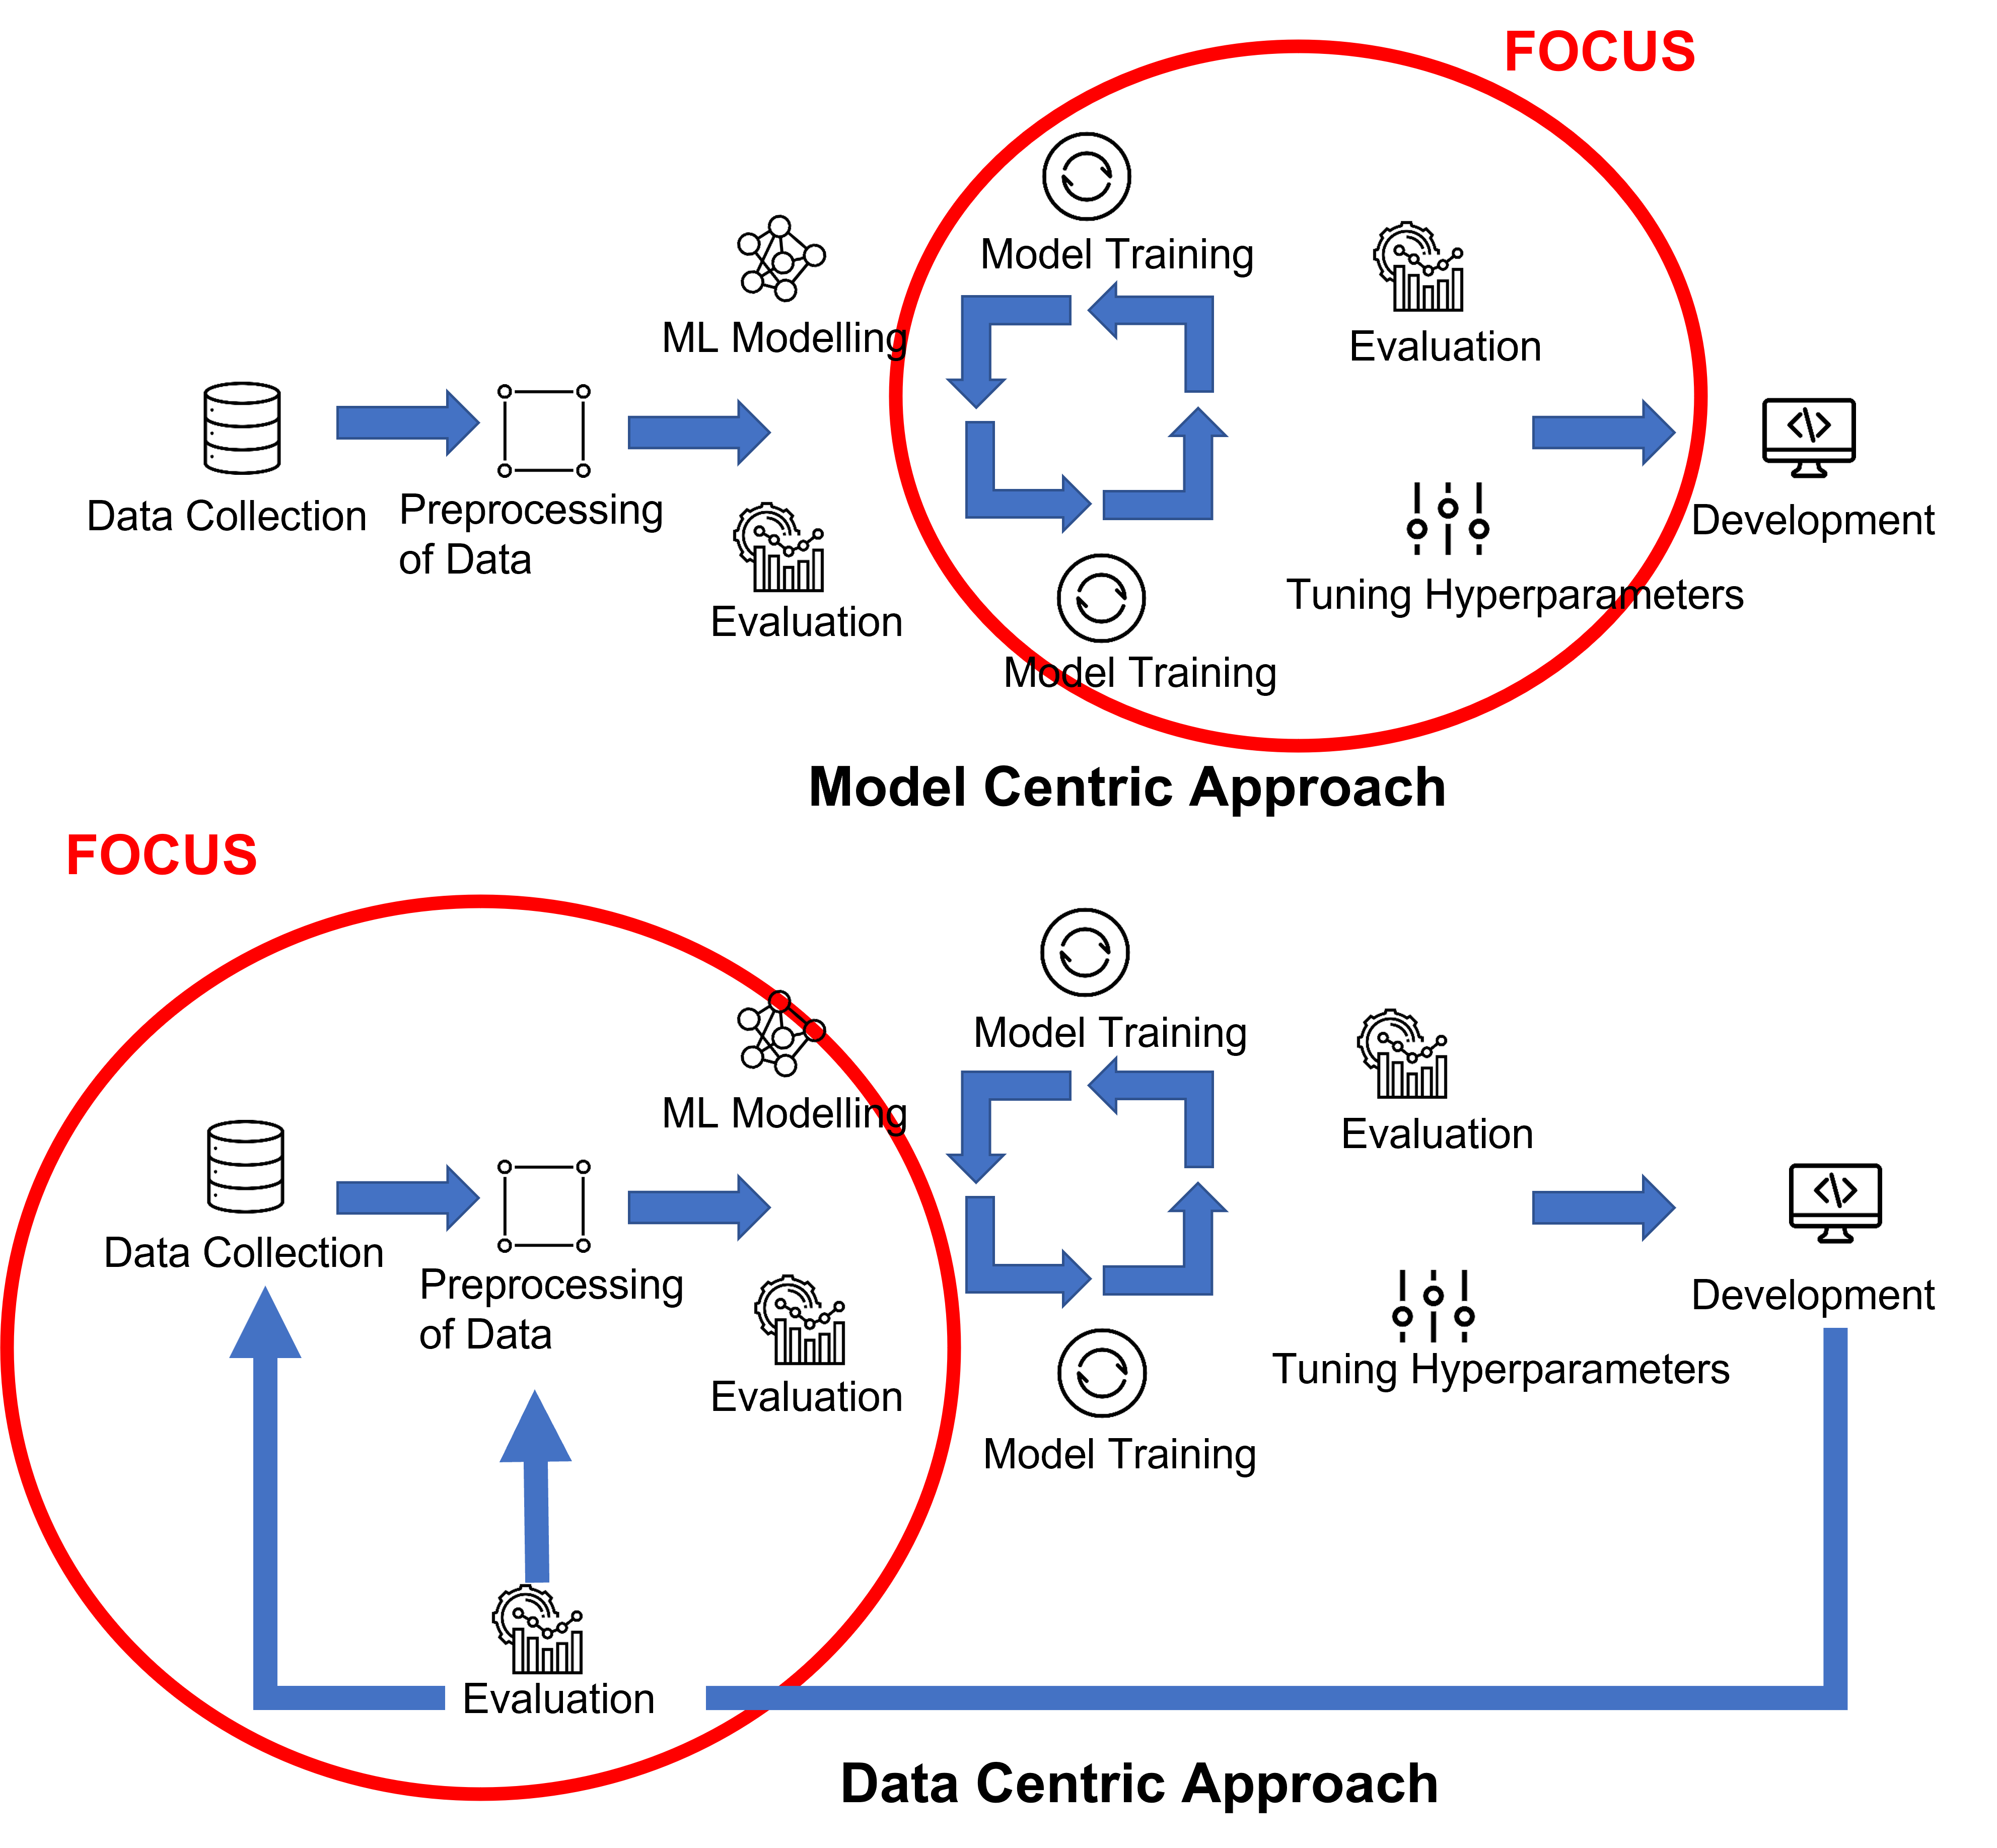
\includegraphics[width=0.7\textwidth]{img/datacentervsmlcenter - 2.png}
    \caption{Data-Centric Vs Model-Centric Approach}
    \label{fig:datacent-vs-modelcent}
\end{figure}

In the implementation of data-centric approach following steps are important \cite{radecic_data-centric_2022}:
\begin{enumerate}
    \item \textbf{Iterative Collection of Data} - Data collection is an iterative process in a data-centric approach, particularly for companies that do not have millions of data points or sources, thus, improving the performance of AI systems as well as the quality and quantity of data.
    \item \textbf{Iterative evaluations} for Data Drift Detection  
    \item \textbf{Quality Data Labelling:} Labelling is often done manually which means human errors and biases will exist. If there are inconsistencies w.r.t how the human experts approach particular problem, machines are not likely to detect those inconsistencies. For this we need to ensure that: 
    \begin{enumerate}[label=(\alph*)]
        %\item \textbf{Multiple labelers, editors and auditors to spot inconsistencies}  
        \item Labelling instructions to be defined and the process to be improved with time and implemented accordingly. 
        \item Inclusion of domain knowledge and expertise.
        \item Maintaining Control of labelling annotation process.
    \end{enumerate}
    \item \textbf{Data Augmentation} - It describes techniques for increasing the number of data points in your sample or the number of defective production parts, by \textit{generating the unseen data} that your model has not seen during the training time and \textit{Removing or adding the noisy observations for adding variance}. We also played around with the speed of data, make changes to pitch or tone, length, adding silences or extra noises using audio editing tools \cite{noauthor_linux_nodate} which added variety.        
\end{enumerate}

Based on above, we decided to take a more Data-Centric Approach where our focus is on making quality Data-set instead of Model Centric approach to Machine Learning as shown in Figure \ref{fig:datacent-vs-modelcent}.





